% $Id: gui_preproc.tex 395 2011-11-17 22:34:59Z cphillip $
%
% Written by Jessica Schrouff
%_______________________________________________

\chapter{Prepare feature set}
\label{chap:PrepFeat}
\minitoc

\section{Introduction}
%===============
\label{sec:prep_intro}
One of the main inputs of a machine learning algorithm consists in a $N_{samples} \times N_{features}$ data matrix, containing the values of selected features for each sample. 
This matrix can either be input directly into the machine or be used to compute a ``similarity matrix", or kernel, of size $N_{samples} \times N_{samples}$, which is then input into the classification/regression algorithm [see ``kernel trick" \cite{Hofmann2008,Aizerman1964}]. PRoNTo computes a linear kernel (i.e. dot product) between the samples.
The `Prepare Feature Set' step computes both the feature and linear kernel matrices from one or more modalities, as defined in the previously built dataset (see chapter \ref{chap:DataDesign}). 
It allows detrending the features in the case of time series (such as fMRI) and scaling each image by a constant factor (input by the user) in the case of quantitative modalities (such as PET). Masks can be specified to perform the classification/regression on specific voxels only (e.g. Regions of Interest).

Multiple runs entered as different modalities (e.g. modality 1 is `fMRI\_run1', modality 2 is `fMRI\_run2',...) can be concatenated in terms of samples during this step. 
The images from different runs should then have the same number of features (i.e. selected voxels). In addition, version 2.0 allows to build multiple kernels, either from multiple modalities, or based on different anatomically labelled regions as defined by an atlas. In the case of multiple modalities, it is required that the selected modalities have the same number of samples, i.e. images. 

\section{Methods and resources}
%========================

After the selection of the dataset and of which modality to include in the feature set (further referred to as FS), the toolbox accesses each image, i.e. it gets the value of the voxels which are comprised in the first level mask selected for that modality (mask specified at the data and design step, see chapter `Data and Design'). 
This access is performed by `blocks' of features, not to overload the RAM memory. In the case of time-series, the user can specify detrending
methods and parameters to apply to the time course of each feature. Methods comprise a polynomial detrending (parameter: order of the polynomial) or
a Discrete Cosine Transform high-pass filter (SPM, parameter: frequency cutoff in seconds). An example of a linear detrending (polynomial detrending
of order 1) is shown in Fig. \ref{fig:lindetrend}.
\begin{figure}[!h]
  \begin{center}
      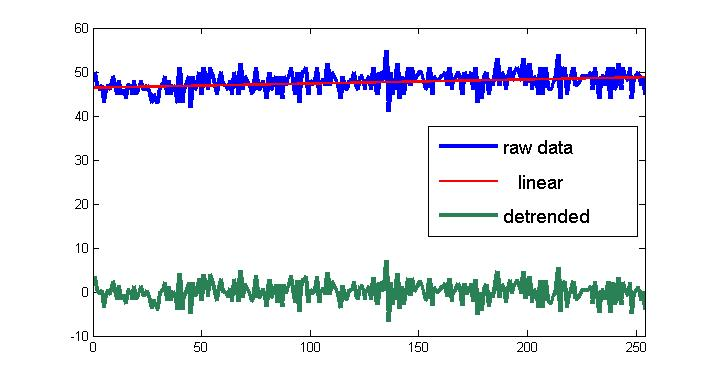
\includegraphics[height=6cm]{images/fig1_lindetrend.png}
   \caption{Example of detrending: the original signal over time of one feature (in blue) was approximated by a polynomial of order 1 (red line), which was then substracted from the original signal to give the detrended signal (in green).}
    \label{fig:lindetrend}
  \end{center}
\end{figure}

For each modality, the (detrended) features are then written in a file array (SPM, with a `.dat' extension), on the hard drive (in the same directory as the dataset). Please note that in the case of large datasets, this operation may require many Gb of free space on the hard drive and long computational times. Therefore, if the first condition can't be fulfilled, we recommend the use of external drives for the whole analysis. Regarding the computational expenses, we tried to minimize their effect by computing the features only once per modality: when preparing other feature sets using the same modality and detrending parameters, the built file array will be accessed for the next steps. 

{\bf Be careful} that using the same modality but different detrending methods and/or parameters will force the re-computation of the file array for the considered modality. In the same way, changing the dataset ({\tt PRT.mat}) from directory might lead to the re-computation of the feature sets if the file arrays were not moved accordingly. 

From the feature set(s), a linear kernel can then be computed. Different options can be specified:
\begin{itemize}
\item All scans/ All conds: In `all scans' the kernel matrix will be computed between all scans within the time series of all subjects and in `all
conds' the kernel matrix is computed only between the scans corresponding to the specified conditions of interest (see `Data and Design'). By default, the toolbox will use all scans to compute the kernel. With large datasets however, computational expenses can be reduced by selecting the last option. 
\item Scaling: allows the specification of constant values to scale each scan. The user has to enter a .mat containing a variable called `scaling' and of the same size as the number of scans in that modality. In case of quantitative modalities such as PET, this step is required since it insures the convergence of the machine learning algorithm.
\item Additional mask for selected modality: this option allows  the specification of a `second-level' mask, which would for example define Regions of Interest (ROIs) on which the classification/regression can be performed. In this case, the voxels used to compute the kernel (and only the kernel) would be the ones contained in both the first and second-level masks. Therefore, using one first-level mask and two second-level masks would create two kernels but only one file array.
\item Build one kernel per region: starting from version v2.0, PRoNTo allows to build one kernel per region as defined by an anatomically defined atlas, specified by the user\footnote{The atlas corresponds to a mask, except that the value of the voxels in each defined area correspond to a unique value, e.g. all voxels in fusiform have the value 3, and all voxels in orbito-frontal have the value 50.}. One atlas (Anatomical Automatic Labelling, AAL) is provided in \textit{your PRoNTo folder/atlas}. Atlases can be generated easily through SPM, or manually by the user. There are no constraints on how regions are built, as long as all the voxels within each region have a specific integer value. The toolbox will identify the different regions based on the values in the voxels. Each region will then act as a second-level mask and one kernel will be built for each region. The kernels are all saved in a same feature set and will then all be used at the modelling stage.
\end{itemize}

These options are performed at the kernel level only. This means that any change in one of these options would lead to the computation of a new kernel but not to the (re)computation of the file arrays. The use of different second-level masks or scaling parameters can therefore be easily envisaged.

ProNTo version 2.0 allows to build multiple kernels. These kernels can be derived from multiple modalities or from multiple regions of interest as defined by an atlas within each modality. These two options are not mutually exclusive and it is also possible to build multiple kernels within each modality and then combine those modalities as multiple kernels. The number of kernels would hence become \textit{number of modalities} $\times$ \textit{number of regions}. In the same way, it is possible to concatenate multiple runs of an experiment while building one kernel per region.

The {\tt PRT.mat} structure saves all information linked to the file arrays in a {\tt fas} field (standing for ``File Array Structure''), which size corresponds to the number of selected modality in all feature sets. The selected options and the link to the kernel (saved on the disk as a .mat) are stored in a {\tt fs} field (standing for ``Feature Set''), which size corresponds to the number of feature sets defined by the user.

\section{Graphical User interfaces}
%==========================

After clicking on the ``Prepare Feature Set'' button in the main interface (see Fig. \ref{fig:mainprep}), a second window will appear (Fig. \ref{fig:FSmainl}), allowing the user to select a saved PRT.mat, to name the FS and to define the number of modalities which should be included in the FS. 
\begin{figure}[!h]
  \begin{center}
      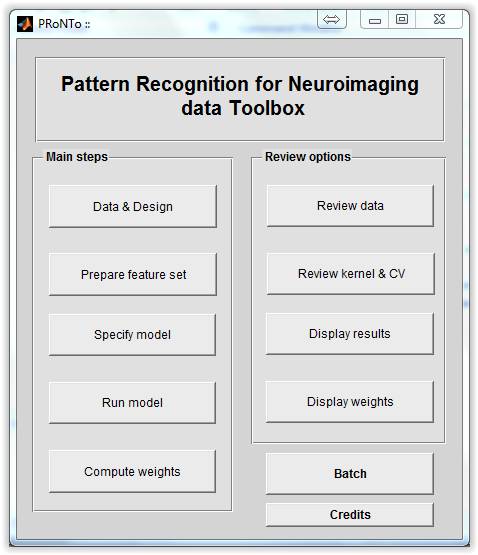
\includegraphics[height=7cm]{images/fig2_main_prt.png}
   \caption{Main interface: button to launch the 'Prepare Feature Set' step.}
    \label{fig:mainprep}
  \end{center}
\end{figure}

\begin{figure}[!h]
  \begin{center}
      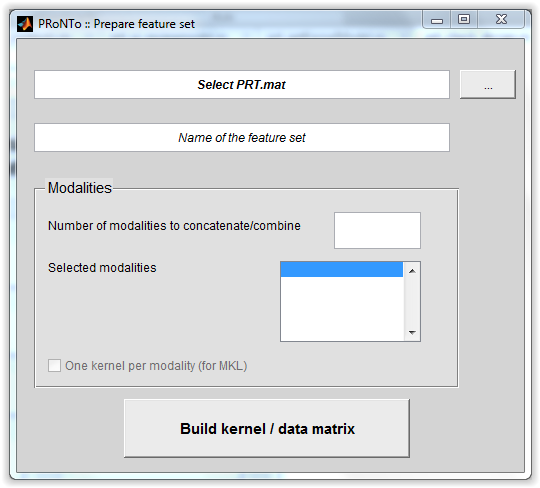
\includegraphics[height=9cm]{images/prt_ui_feature_set.PNG}
   \caption{Interface of the `Prepare Feature Set' step. Top: Dataset selection: type the full name (with path) or browse to select the dataset to prepare. Feature set name: Type the FS name, which will be used to save the kernel as a .mat on the hard drive. Modalities: Number of modalities to select with the list containing the names of the modalities included in the FS (no user interaction possible). A checkbox allows to build one kernel per modality if multiple modalities are present/have been selected in the FS. Build kernel/data matrix: builds the feature set and kernel(s).}
    \label{fig:FSmainl}
  \end{center}
\end{figure}

To define the number of modalities to include, the user should click in the appropriate edit box, type the number and then `return'. This will launch a third window (Fig. \ref{fig:modFS}), allowing the specification of the different options and parameters for each modality. When the dataset contains only one modality, this window is launched directly and (Fig. \ref{fig:FSmainl}) is filled automatically expect for the feature set name.
\begin{figure}[!h]
  \begin{center}
      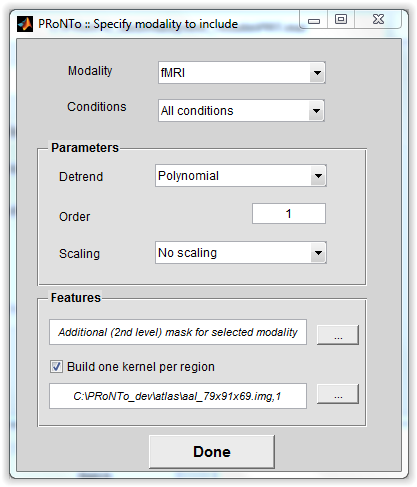
\includegraphics[height=7cm]{images/prt_ui_feature_set_modality.PNG}
   \caption{Specification of options and parameters for each modality. Modality: Select the modality name from a pull-down menu. Conditions: choose to build All scans or All conditions. Parameters: Detrend to perform with its parameter, as well as Scaling of the scans or not. Features: Selection of a second-level mask and/or of an atlas to build one kernel per region.}
    \label{fig:modFS}
  \end{center}
\end{figure}

In this third window, the user has to choose which modality to include based on its name (first pull-down menu) and  which scans to use to build the kernel (all or only those linked to the design). All other options are facultative. The first panel refers to operations to perform on the features:
\begin{itemize}
\item the detrending parameters: by default, the parameter is set to `No detrending'. However, we recommend to perform a detrending in the case of
time series data such as fMRI (and only in that case). When selecting polynomial, the `order' parameter will appear, with a default value of 1.
Changing this value will increase the order of the polynomial used to fit the data. If `Discrete Cosine Transform' is selected, the editable
parameter corresponds to the cutoff frequency (in seconds) of the high-pass filter. Please note that, when including more than one run (`modality') into a feature set, nothing will prevent the user from using different detrending methods/parameters. We however highly recommend to use a consistent detrending in the same FS.
\item the scaling: `no scaling' is the default option. However, when dealing with quantitative modalities such as PET, the user should provide one value per scan, stored in a vector in a .mat file under the variable name 'scaling'.
\end{itemize}

As previously mentioned, the detrending is performed before the features are saved in the file array, while the scaling is performed only when building the kernel.

The second panel allows to select a subset of the saved features to build the kernel. Two options are available:
\begin{itemize}
\item the specification of a second-level mask: type the full name (with path) of the mask or browse to select the mask image. When left empty or untouched, voxels are selected from the first-level mask specified in the data and design step. Otherwise, voxels within both the first and second-level masks will be selected to build the kernel.
\item the building of one kernel per region: when selecting this option, the user should load an atlas which defines regions in terms of their anatomy (in MNI space). Each region will then act as a second-level mask and one kernel will be built for each region. 
\end{itemize}

When working with Graphical User Interfaces (GUIs), some messages might appear in \matlab workspace. These can display information about the operations currently performed or explain why the toolbox does not do as the user expected (e.g. when a file could not be loaded or if information was input in a wrong format). Therefore we strongly encourage the user to have a look at \matlab prompt when using GUIs.

\section{{\tt matlabbatch} interface}
%=======================

The {\tt matlabbatch} system allows the input/selection of all parameters and options aforementioned. Just note that the batch is based on the names of the modalities and/or conditions. Therefore, for the batch to work properly, names should be consistent across all steps, starting from data and design to the model specification and running. The hierarchy for the case of a feature set containing one fMRI modality is displayed in (Fig. \ref{fig:batchFS}). For this feature set, we chose to load an atlas, and build multiple kernels based on the regions it defines.

\begin{figure}[!h]
  \begin{center}
      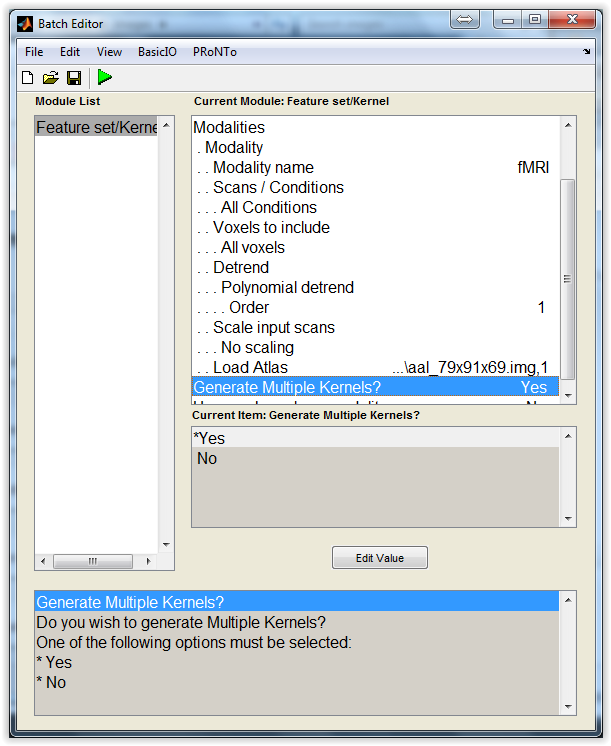
\includegraphics[height=10cm]{images/fig5_batchFS.png}
   \caption{{\tt matlabbatch} GUI for feature set building.}
    \label{fig:batchFS}
  \end{center}
\end{figure}

{\bf Important note:} Defining all important steps in one batch and running that batch will overwrite the {\tt PRT.mat} previously created and thus delete the links between the {\tt PRT.mat} and the computed kernel(s) and feature set(s). The file arrays would then be recomputed each time the batch is launched. For large datasets, we therefore recommend splitting the batch in two parts: a data and design and prepare feature set part and a second part comprising the model specification, run model and compute weights modules. This would indeed allow changing, e.g. model parameters, without recomputing the feature sets and kernels. 
